\documentclass{article}
\usepackage{fullpage} % sets more standardized margins
\usepackage{graphicx} % some graphics functions I use 
\usepackage{abstract} % abstract function
\usepackage{amsmath}  % math stuff
\usepackage{float}
\usepackage{mathrsfs}
\usepackage[utf8]{inputenc}
\usepackage[document]{ragged2e}
\usepackage{subfiles}
\usepackage{caption}
\usepackage{subcaption}
\usepackage{verbatim}
\usepackage[toc,page]{appendix}

\renewcommand{\absnamepos}{flushleft} % left justifies abstract
\setlength{\absleftindent}{0pt}
\setlength{\absrightindent}{0pt}



% % %
% Set up IEEE style paragraphing
% % %
\setlength{\parskip}{1em} % The \par command now skips a line between paragraphs, eliminates warnings from using the \par or \\ commands
\setlength{\parindent}{0em} % Left justifies paragraphs after a \par command 


\begin{document}

\pagenumbering{gobble} % Turn off page numbering for titles and tables


\begin{titlepage}
    \begin{center}
        
         \vspace*{1.5cm}
        
    %Berkay suggested this title in the meeting
         \textbf{{\Huge Proposal: }}
        
         \vspace{0.5cm}
         \textbf{Application of IR-transmitter As IR Tripwire}
        
          \vspace{.5cm}
        
         \textbf{{\Large Joseph Arsenault \\ Ryan Dufour \\ Phil Robb \newline}}
    \vspace{.4cm}
    	
    	\textbf{joseph.m.arsenault@maine.edu \\ ryan.dufour@maine.edu \\ phil.robb@maine.edu}
    	
    \vspace{1cm}
    
        
        
        \begin{abstract}
        
        
        %I re-worded it here, check it over to make sure it sounds not so choppy and details what is needed
        
        \noindent 
       An infrared tripwire is proposed as a novel and useful application for the transmitter and receiver modules of the Optical Uplink project. The importance of efficient and non-intrusive trip wire sensors for both defense and retail applications is outlined, in addition, the background theory for infrared sensors is described. Preliminary measured results of the Optical Uplink are provided as well as their ramifications on the tripwire sensor are discussed. Relevant qualifications of all team members is described and sufficient experience is with required technology is shown. Finally, a cost analysis for design and production of the proposed tripwire is performed.
        
        
        
        %An LF347 wide bandwidth quad JFET input operational amplifier integrated circuit, MFBP filter, with rail voltages of $\pm$12V, was used to amplify the output signal from a transimpedance amplifier. This is used as a module for an optical uplink circuit. The filter is required to have a center frequency of 20kHz, a 3dB bandwidth between 1.5kHz and 5kHz, a gain of greater than 60dB, and rail supplies of $\pm$12V. A sinusoidal waveform with an amplitude of 100mV and frequency of 20kHz was used for the input to the MFBP filter. The output voltage operated with a gain of 71.4dB, with a bandwidth at 3dB of 2.11kHz and a center frequency of 20.2kHz. 
        \end{abstract}
        
        
        \vspace{02.5cm}
        \textbf{
        Electrical and Computer Engineering\\
        University of Maine\\
        ECE - 342\\\ \today}
    \vspace{.5cm}
    
    \end{center}
\end{titlepage}


\tableofcontents

\newpage

\newpage
\listoffigures
\listoftables
\newpage 
\clearpage

\pagenumbering{arabic} % Turn on page numbering



\section{Introduction}
\subfile{Introduction/Introduction}
  
 
  \section{Background}
    \subfile{Background/Circuit.tex}
  
   \section{Proposed Work}
   	\subfile{Proposed_work/Simulations.tex} 
 	
    
  \section{Preliminary Results}
  	\subfile{Preliminary_results/experimental.tex}

    
  \section{Team Qualifications}
     \subfile{Team_qualifications/Discussion.tex}
    
    
    
   \section{Cost Analysis}
   	\subfile{Cost_Analysis/cost.tex}
   	
    \section{Conclusion}
        \subfile{Conclusion/Conclusion.tex}

    
    \newpage
\clearpage

\appendix

\begin{thebibliography}{00}



\bibitem{b1} Doug Richardson. (2002) "Sensors, Sentry Owls and smart dust: since the summer of 2002, Sentry Owls have been helping guard US units operating in overseas locations close to Afghanistan." Business Insights: Essentials. 
\newline

\bibitem{b2} A. A. Faust, et Al. (2005) "Canadian teleoperated landmine detection systems." Avalable: Internation Journal of System Sciences.
\newline

\bibitem{b3} Vicaire, Pascal, et Al. (2009) "Acheiving Long-term Surveillance in VigilNet." Available: ACM Trans. Sen. Netw.
\newline

\newpage


\end{thebibliography}

\begin{appendices}
	

\begin{figure}[H]
	\centering
	\caption[NRE Costs]{}
	\label{fig:costanalysis}
	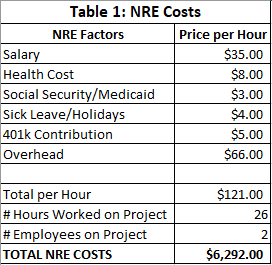
\includegraphics[width=0.5\linewidth]{costanalysis}
\end{figure}

\begin{figure}[H]
	\centering
	\caption[Assembly Costs]{}
	\label{fig:assmcosts}
	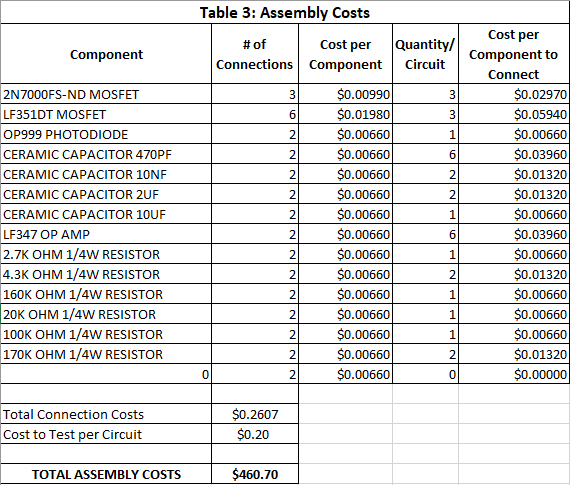
\includegraphics[width=0.5\linewidth]{assmcosts}
\end{figure}

\begin{figure}[H]
	\centering
	\caption[Component Costs]{}
	\label{fig:compcost}
	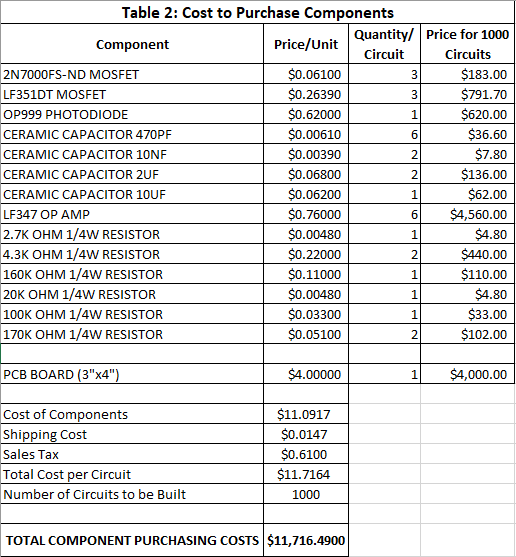
\includegraphics[width=0.5\linewidth]{compcost}
\end{figure}

\end{appendices}




\begin{comment}
\section{References}

\noindent [1] N.W. Emanatoglu.(2017) Lab $\#1$; photodetector and transimpedence amplifier [Online]. Available: http://web.eece.maine.edu/~kotecki/ECE342/labs/ECE342_2017_Lab2.pdf
\newline

\noindent [2] D.E. Kotecki Lab.(2017) Resistively Loaded MOSFET Gate [Online]. Available: http://web.eece.maine.edu/~kotecki/ECE342/labs/ECE342_2017_Lab3_Inverter.pdf
\newline

\noindent [3] N.W. Emanatoglu.(2017) Lab $\#1$; photodetector and transimpedence amplifier [Online]. Available: http://web.eece.maine.edu/~kotecki/ECE342/labs/ECE342_2017_Lab2_MFBF.pdf
\newline

\noindent [4] Cree.(2014) 5-mm Blue and Green LED [Online]. Available http://www.cree.com/led-components/media/documents/C503B-BAS-BAN-BCS-BCN-GAS-GAN-GCS-GCN-1094.pdf
\newline

\noindent [5] Kingbright.(2017) WP7113SGC [Online]. Available: http://www.us.kingbright.com/images/catalog/SPEC/WP7113SGC.pdf
\newline

\noindent [6] D.E. Kotecki Lab.(2017) PIN Silicon Photodiode [Online]. Available: http://web.eece.maine.edu/~kotecki/ECE342/datasheets/OP993-999\_0.pdf
\newline

\noindent [7] Kingbright.(2017) WP7113SEC/J3 [Online]Available: http://www.kingbrightusa.com/images/catalog/SPEC/WP7113SEC-J3.pdf
\newline

\noindent [8] Everlight.(2006) IR1503 [Online]. Available: https://radiodetali.com/media/catalog/product/i/r/ir1503.pdf
\newline
\end{comment}

\end{document}
